\section{Meta\-Bundle Class Reference}
\label{classMetaBundle}\index{MetaBundle@{MetaBundle}}
{\tt \#include $<$metabundle.h$>$}

\subsection*{Public Member Functions}
\begin{CompactItemize}
\item 
{\bf Meta\-Bundle} ()
\item 
{\bf Meta\-Bundle} (const KURL \&u)
\item 
{\bf Meta\-Bundle} (const QString \&title, const QString \&stream\-Url, const int bitrate, const QString \&genre, const QString \&stream\-Name, const KURL \&)
\item 
{\bf Meta\-Bundle} (const KURL \&url, Tag\-Lib::Tag $\ast$tag, Tag\-Lib::Audio\-Properties $\ast$ap=0)
\item 
{\bf Meta\-Bundle} \& {\bf read\-Tags} (bool audio\-Properties=true)
\item 
int {\bf length} () const 
\item 
int {\bf bitrate} () const 
\item 
int {\bf sample\-Rate} () const 
\item 
bool {\bf exist} ()
\item 
const KURL \& {\bf url} () const 
\item 
const QString \& {\bf title} () const 
\item 
const QString \& {\bf artist} () const 
\item 
const QString \& {\bf album} () const 
\item 
const QString \& {\bf year} () const 
\item 
const QString \& {\bf comment} () const 
\item 
const QString \& {\bf genre} () const 
\item 
const QString \& {\bf track} () const 
\item 
QString {\bf pretty\-Title} () const 
\item 
QString {\bf pretty\-URL} () const 
\item 
QString {\bf pretty\-Bitrate} () const 
\item 
QString {\bf pretty\-Length} () const 
\item 
QString {\bf pretty\-Sample\-Rate} () const 
\end{CompactItemize}
\subsection*{Static Public Member Functions}
\begin{CompactItemize}
\item 
QString {\bf pretty\-Bitrate} (int)
\item 
QString {\bf pretty\-Length} (int)
\item 
QString {\bf pretty\-Time} (int, bool show\-Hours=true)
\item 
QString {\bf zero\-Pad} (uint i)
\item 
QString {\bf pretty\-Title} (QString)
\end{CompactItemize}
\subsection*{Static Public Attributes}
\begin{CompactItemize}
\item 
const int {\bf Undetermined} = -2
\item 
const int {\bf Irrelevant} = -1
\item 
const int {\bf Unavailable} = 0
\end{CompactItemize}
\subsection*{Private Member Functions}
\begin{CompactItemize}
\item 
void {\bf init} (Tag\-Lib::Audio\-Properties $\ast$ap=0)
\item 
void {\bf init} (const KFile\-Meta\-Info \&info)
\end{CompactItemize}
\subsection*{Static Private Member Functions}
\begin{CompactItemize}
\item 
QString {\bf pretty\-Generic} (const QString \&, int)
\end{CompactItemize}
\subsection*{Private Attributes}
\begin{CompactItemize}
\item 
KURL {\bf m\_\-url}
\item 
QString {\bf m\_\-title}
\item 
QString {\bf m\_\-artist}
\item 
QString {\bf m\_\-album}
\item 
QString {\bf m\_\-year}
\item 
QString {\bf m\_\-comment}
\item 
QString {\bf m\_\-genre}
\item 
QString {\bf m\_\-track}
\item 
int {\bf m\_\-bitrate}
\item 
int {\bf m\_\-length}
\item 
int {\bf m\_\-sample\-Rate}
\item 
bool {\bf exists}
\end{CompactItemize}


\subsection{Constructor \& Destructor Documentation}
\index{MetaBundle@{Meta\-Bundle}!MetaBundle@{MetaBundle}}
\index{MetaBundle@{MetaBundle}!MetaBundle@{Meta\-Bundle}}
\subsubsection{\setlength{\rightskip}{0pt plus 5cm}Meta\-Bundle::Meta\-Bundle ()\hspace{0.3cm}{\tt  [inline]}}\label{classMetaBundle_MetaBundlea0}




Definition at line 33 of file metabundle.h.

References init().



\footnotesize\begin{verbatim}33 { init(); }
\end{verbatim}\normalsize 


Here is the call graph for this function:\begin{figure}[H]
\begin{center}
\leavevmode

\includegraphics[width=145pt]{classMetaBundle_MetaBundlea0_cgraph}
\end{center}
\end{figure}
\index{MetaBundle@{Meta\-Bundle}!MetaBundle@{MetaBundle}}
\index{MetaBundle@{MetaBundle}!MetaBundle@{Meta\-Bundle}}
\subsubsection{\setlength{\rightskip}{0pt plus 5cm}Meta\-Bundle::Meta\-Bundle (const KURL \& {\em u})\hspace{0.3cm}{\tt  [inline]}}\label{classMetaBundle_MetaBundlea1}




Definition at line 34 of file metabundle.h.

References m\_\-url, and read\-Tags().



\footnotesize\begin{verbatim}34 : m_url( u ) { readTags(); }
\end{verbatim}\normalsize 


Here is the call graph for this function:\begin{figure}[H]
\begin{center}
\leavevmode
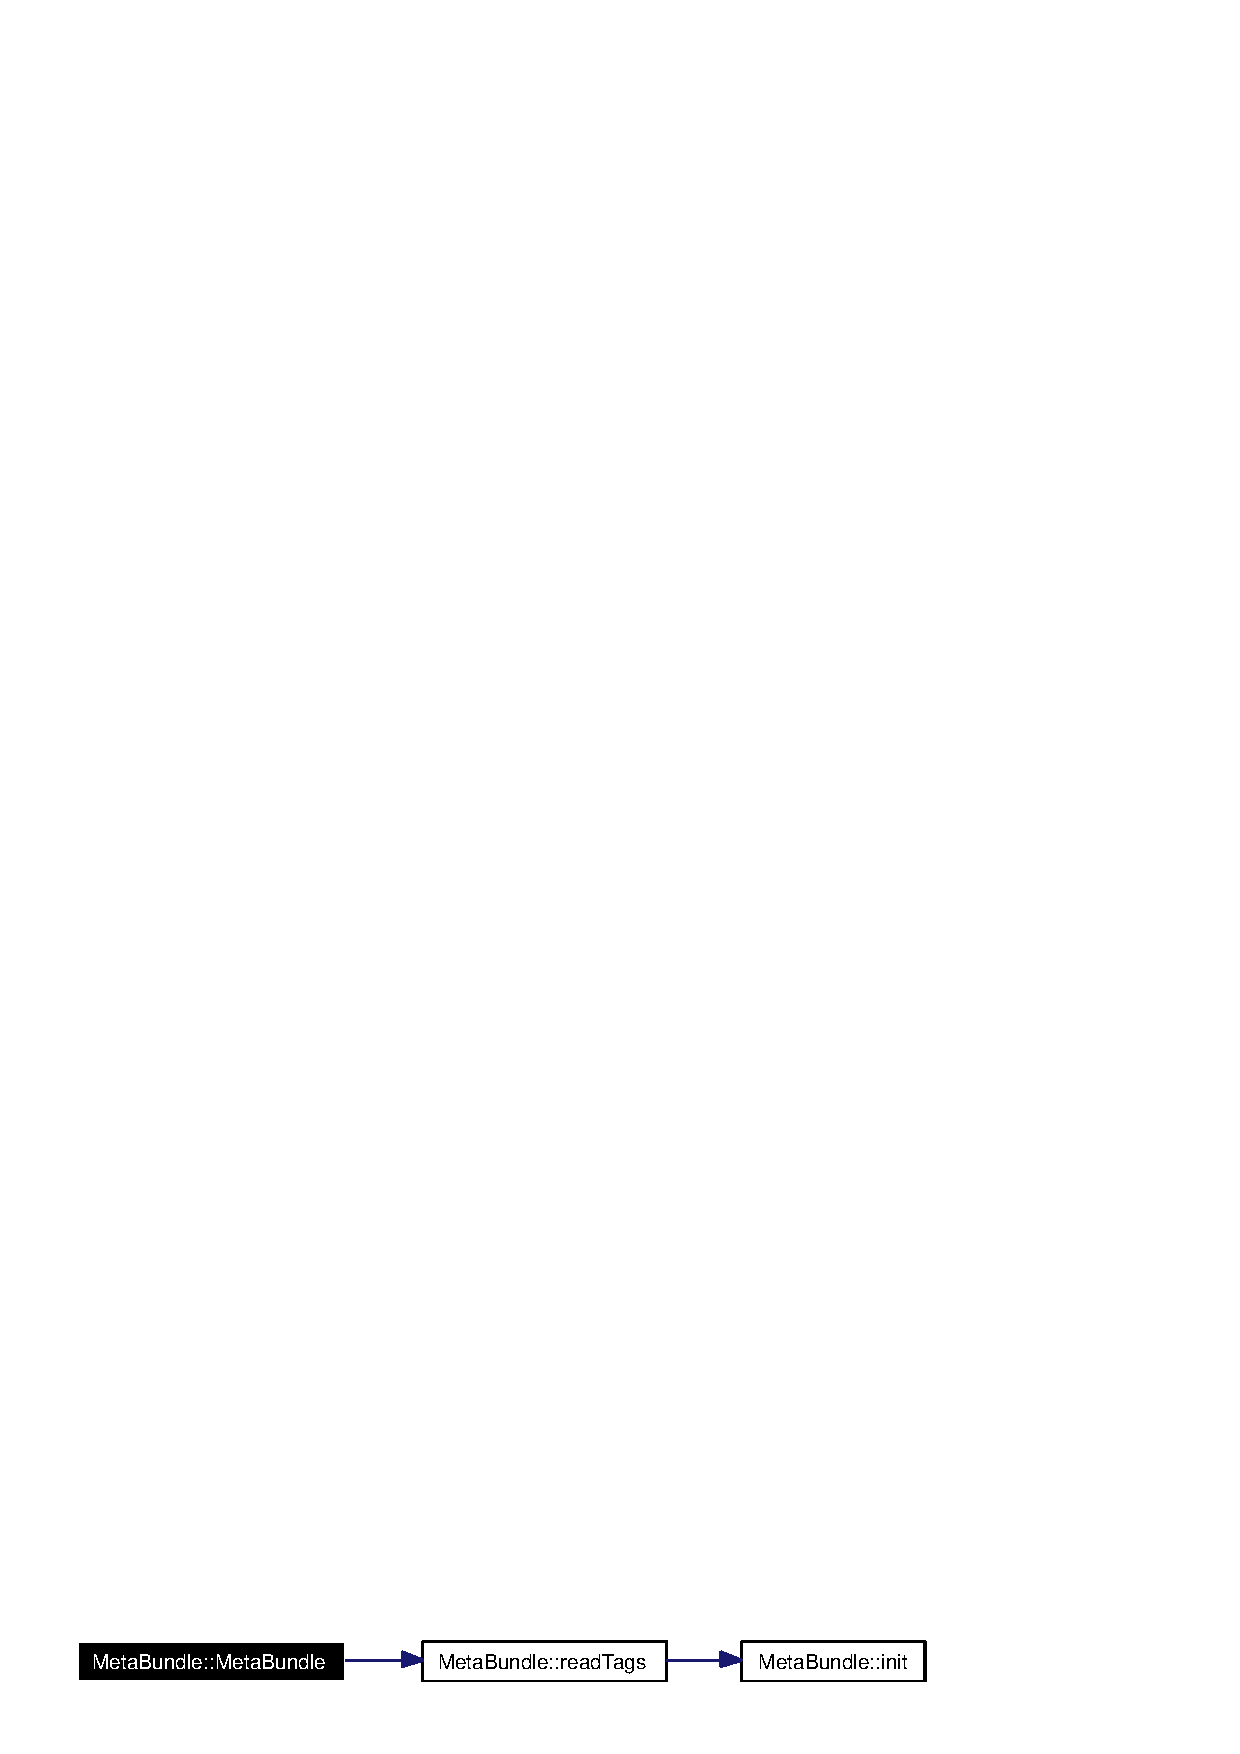
\includegraphics[width=222pt]{classMetaBundle_MetaBundlea1_cgraph}
\end{center}
\end{figure}
\index{MetaBundle@{Meta\-Bundle}!MetaBundle@{MetaBundle}}
\index{MetaBundle@{MetaBundle}!MetaBundle@{Meta\-Bundle}}
\subsubsection{\setlength{\rightskip}{0pt plus 5cm}Meta\-Bundle::Meta\-Bundle (const QString \& {\em title}, const QString \& {\em stream\-Url}, const int {\em bitrate}, const QString \& {\em genre}, const QString \& {\em stream\-Name}, const KURL \&)}\label{classMetaBundle_MetaBundlea2}




Definition at line 39 of file metabundle.cpp.



\footnotesize\begin{verbatim}45   : m_url       ( url )
46   , m_title     ( streamUrl + QString( " -- " ) + title )
47   , m_genre     ( genre )
48   , m_bitrate   ( bitrate )
49   , m_length    ( Irrelevant )
50   , m_sampleRate( Unavailable )
51   ,exists(false)
52 {
53 kdDebug() << "Test point 1 " << endl;
54 }
\end{verbatim}\normalsize 
\index{MetaBundle@{Meta\-Bundle}!MetaBundle@{MetaBundle}}
\index{MetaBundle@{MetaBundle}!MetaBundle@{Meta\-Bundle}}
\subsubsection{\setlength{\rightskip}{0pt plus 5cm}Meta\-Bundle::Meta\-Bundle (const KURL \& {\em url}, Tag\-Lib::Tag $\ast$ {\em tag}, Tag\-Lib::Audio\-Properties $\ast$ {\em ap} = 0)}\label{classMetaBundle_MetaBundlea3}




Definition at line 96 of file metabundle.cpp.

References init().



\footnotesize\begin{verbatim}97   : m_url( url )
98   , m_title(   TStringToQString( tag->title() ).stripWhiteSpace() )
99   , m_artist(  TStringToQString( tag->artist() ).stripWhiteSpace() )
100   , m_album(   TStringToQString( tag->album() ).stripWhiteSpace() )
101   , m_year(    tag->year() ? QString::number( tag->year() ) : QString::null )
102   , m_comment( TStringToQString( tag->comment() ).stripWhiteSpace() )
103   , m_genre(   TStringToQString( tag->genre() ).stripWhiteSpace() )
104   , m_track(   tag->track() ? QString::number( tag->track() ) : QString::null )
105   ,exists(false)
106 {
107 kdDebug() << "Test point 2 " << endl;
108     init( ap );
109 }
\end{verbatim}\normalsize 


Here is the call graph for this function:\begin{figure}[H]
\begin{center}
\leavevmode

\includegraphics[width=145pt]{classMetaBundle_MetaBundlea3_cgraph}
\end{center}
\end{figure}


\subsection{Member Function Documentation}
\index{MetaBundle@{Meta\-Bundle}!album@{album}}
\index{album@{album}!MetaBundle@{Meta\-Bundle}}
\subsubsection{\setlength{\rightskip}{0pt plus 5cm}const QString\& Meta\-Bundle::album () const\hspace{0.3cm}{\tt  [inline]}}\label{classMetaBundle_MetaBundlea12}




Definition at line 61 of file metabundle.h.

References m\_\-album.

Referenced by Myplayer::handle\-Message().



\footnotesize\begin{verbatim}61 { return m_album; }
\end{verbatim}\normalsize 
\index{MetaBundle@{Meta\-Bundle}!artist@{artist}}
\index{artist@{artist}!MetaBundle@{Meta\-Bundle}}
\subsubsection{\setlength{\rightskip}{0pt plus 5cm}const QString\& Meta\-Bundle::artist () const\hspace{0.3cm}{\tt  [inline]}}\label{classMetaBundle_MetaBundlea11}




Definition at line 60 of file metabundle.h.

References m\_\-artist.

Referenced by Myplayer::handle\-Message().



\footnotesize\begin{verbatim}60 { return m_artist; }
\end{verbatim}\normalsize 
\index{MetaBundle@{Meta\-Bundle}!bitrate@{bitrate}}
\index{bitrate@{bitrate}!MetaBundle@{Meta\-Bundle}}
\subsubsection{\setlength{\rightskip}{0pt plus 5cm}int Meta\-Bundle::bitrate () const\hspace{0.3cm}{\tt  [inline]}}\label{classMetaBundle_MetaBundlea6}




Definition at line 55 of file metabundle.h.

References m\_\-bitrate.

Referenced by Myplayer::handle\-Message().



\footnotesize\begin{verbatim}55 { return m_bitrate; }
\end{verbatim}\normalsize 
\index{MetaBundle@{Meta\-Bundle}!comment@{comment}}
\index{comment@{comment}!MetaBundle@{Meta\-Bundle}}
\subsubsection{\setlength{\rightskip}{0pt plus 5cm}const QString\& Meta\-Bundle::comment () const\hspace{0.3cm}{\tt  [inline]}}\label{classMetaBundle_MetaBundlea14}




Definition at line 63 of file metabundle.h.

References m\_\-comment.



\footnotesize\begin{verbatim}63 { return m_comment; }
\end{verbatim}\normalsize 
\index{MetaBundle@{Meta\-Bundle}!exist@{exist}}
\index{exist@{exist}!MetaBundle@{Meta\-Bundle}}
\subsubsection{\setlength{\rightskip}{0pt plus 5cm}bool Meta\-Bundle::exist ()}\label{classMetaBundle_MetaBundlea8}




Definition at line 256 of file metabundle.cpp.

References exists.



\footnotesize\begin{verbatim}257 {
258         return exists;
259 }\end{verbatim}\normalsize 
\index{MetaBundle@{Meta\-Bundle}!genre@{genre}}
\index{genre@{genre}!MetaBundle@{Meta\-Bundle}}
\subsubsection{\setlength{\rightskip}{0pt plus 5cm}const QString\& Meta\-Bundle::genre () const\hspace{0.3cm}{\tt  [inline]}}\label{classMetaBundle_MetaBundlea15}




Definition at line 64 of file metabundle.h.

References m\_\-genre.



\footnotesize\begin{verbatim}64 { return m_genre; }
\end{verbatim}\normalsize 
\index{MetaBundle@{Meta\-Bundle}!init@{init}}
\index{init@{init}!MetaBundle@{Meta\-Bundle}}
\subsubsection{\setlength{\rightskip}{0pt plus 5cm}void Meta\-Bundle::init (const KFile\-Meta\-Info \& {\em info})\hspace{0.3cm}{\tt  [private]}}\label{classMetaBundle_MetaBundled1}




Definition at line 130 of file metabundle.cpp.

References exists, m\_\-album, m\_\-artist, m\_\-bitrate, m\_\-comment, m\_\-genre, m\_\-length, m\_\-sample\-Rate, m\_\-title, m\_\-track, m\_\-url, m\_\-year, pretty\-Title(), and Undetermined.



\footnotesize\begin{verbatim}131 {
132     if( info.isValid() )
133     {
134         exists=true;
135         m_artist     = info.item( "Artist" ).string();
136         m_album      = info.item( "Album" ).string();
137         m_year       = info.item( "Year" ).string();
138         m_comment    = info.item( "Comment" ).string();
139         m_genre      = info.item( "Genre" ).string();
140         m_track      = info.item( "Track" ).string();
141         m_bitrate    = info.item( "Bitrate" ).value().toInt();
142         m_length     = info.item( "Length" ).value().toInt();
143         m_sampleRate = info.item( "Sample Rate" ).value().toInt();
144 
145         /*
146          * For title, check if it is valid. If not, use prettyTitle.
147          * See bug#83650.
148          */
149         KFileMetaInfoItem item = info.item( "Title" );
150         if( item.isValid() )
151             m_title = item.string();
152         else
153             m_title = prettyTitle( m_url.fileName() );
154     }
155     else m_bitrate = m_length = m_sampleRate = Undetermined;
156 }
\end{verbatim}\normalsize 


Here is the call graph for this function:\begin{figure}[H]
\begin{center}
\leavevmode

\includegraphics[width=140pt]{classMetaBundle_MetaBundled1_cgraph}
\end{center}
\end{figure}
\index{MetaBundle@{Meta\-Bundle}!init@{init}}
\index{init@{init}!MetaBundle@{Meta\-Bundle}}
\subsubsection{\setlength{\rightskip}{0pt plus 5cm}void Meta\-Bundle::init (Tag\-Lib::Audio\-Properties $\ast$ {\em ap} = 0)\hspace{0.3cm}{\tt  [private]}}\label{classMetaBundle_MetaBundled0}




Definition at line 112 of file metabundle.cpp.

References exists, m\_\-bitrate, m\_\-length, m\_\-sample\-Rate, m\_\-url, and Undetermined.

Referenced by Meta\-Bundle(), and read\-Tags().



\footnotesize\begin{verbatim}113 {
114     if( !m_url.isLocalFile() )
115      {
116         exists=false;    
117         return;
118     }   
119     if( ap )
120     {
121         m_bitrate    = ap->bitrate();
122         m_length     = ap->length();
123         m_sampleRate = ap->sampleRate();
124     }
125     else m_bitrate = m_length = m_sampleRate = Undetermined;
126     exists=true;
127 }
\end{verbatim}\normalsize 
\index{MetaBundle@{Meta\-Bundle}!length@{length}}
\index{length@{length}!MetaBundle@{Meta\-Bundle}}
\subsubsection{\setlength{\rightskip}{0pt plus 5cm}int Meta\-Bundle::length () const\hspace{0.3cm}{\tt  [inline]}}\label{classMetaBundle_MetaBundlea5}




Definition at line 54 of file metabundle.h.

References m\_\-length.

Referenced by Myplayer::handle\-Message(), and Engine\-Controller::slot\-Main\-Timer().



\footnotesize\begin{verbatim}54 { return m_length > 0 ? m_length : 0; }
\end{verbatim}\normalsize 
\index{MetaBundle@{Meta\-Bundle}!prettyBitrate@{prettyBitrate}}
\index{prettyBitrate@{prettyBitrate}!MetaBundle@{Meta\-Bundle}}
\subsubsection{\setlength{\rightskip}{0pt plus 5cm}QString Meta\-Bundle::pretty\-Bitrate (int)\hspace{0.3cm}{\tt  [static]}}\label{classMetaBundle_MetaBundlee0}




Definition at line 244 of file metabundle.cpp.

References bitrate\-Store, and pretty\-Generic().



\footnotesize\begin{verbatim}245 {
246     return ( i % 32 == 0 && i < 257 ) ? bitrateStore[ i /32 ] : prettyGeneric( i18n( "Bitrate", "%1 kbps" ), i );
247 }
\end{verbatim}\normalsize 


Here is the call graph for this function:\begin{figure}[H]
\begin{center}
\leavevmode

\includegraphics[width=169pt]{classMetaBundle_MetaBundlee0_cgraph}
\end{center}
\end{figure}
\index{MetaBundle@{Meta\-Bundle}!prettyBitrate@{prettyBitrate}}
\index{prettyBitrate@{prettyBitrate}!MetaBundle@{Meta\-Bundle}}
\subsubsection{\setlength{\rightskip}{0pt plus 5cm}QString Meta\-Bundle::pretty\-Bitrate () const\hspace{0.3cm}{\tt  [inline]}}\label{classMetaBundle_MetaBundlea19}




Definition at line 69 of file metabundle.h.

References m\_\-bitrate.



\footnotesize\begin{verbatim}69 { return prettyBitrate( m_bitrate ); }
\end{verbatim}\normalsize 
\index{MetaBundle@{Meta\-Bundle}!prettyGeneric@{prettyGeneric}}
\index{prettyGeneric@{prettyGeneric}!MetaBundle@{Meta\-Bundle}}
\subsubsection{\setlength{\rightskip}{0pt plus 5cm}QString Meta\-Bundle::pretty\-Generic (const QString \&, int)\hspace{0.3cm}{\tt  [static, private]}}\label{classMetaBundle_MetaBundleh0}




Definition at line 250 of file metabundle.cpp.

References Undetermined.

Referenced by pretty\-Bitrate(), and pretty\-Sample\-Rate().



\footnotesize\begin{verbatim}251 {
252     //TODO ensure this inlines
253 
254     return ( i > 0 ) ? s.arg( i ) : ( i == Undetermined ) ? "?" : QString::null;
255 }
\end{verbatim}\normalsize 
\index{MetaBundle@{Meta\-Bundle}!prettyLength@{prettyLength}}
\index{prettyLength@{prettyLength}!MetaBundle@{Meta\-Bundle}}
\subsubsection{\setlength{\rightskip}{0pt plus 5cm}QString Meta\-Bundle::pretty\-Length (int)\hspace{0.3cm}{\tt  [static]}}\label{classMetaBundle_MetaBundlee1}




Definition at line 212 of file metabundle.cpp.

References Irrelevant, pretty\-Time(), and Unavailable.



\footnotesize\begin{verbatim}213 {
214     QString s;
215 
216     if( seconds > 0 ) s = prettyTime( seconds, false );
217     else if( seconds == Unavailable ) s = '?';
218     else if( seconds == Irrelevant  ) s = '-';
219 
220     return s; //Undetermined = ""
221 }
\end{verbatim}\normalsize 


Here is the call graph for this function:\begin{figure}[H]
\begin{center}
\leavevmode
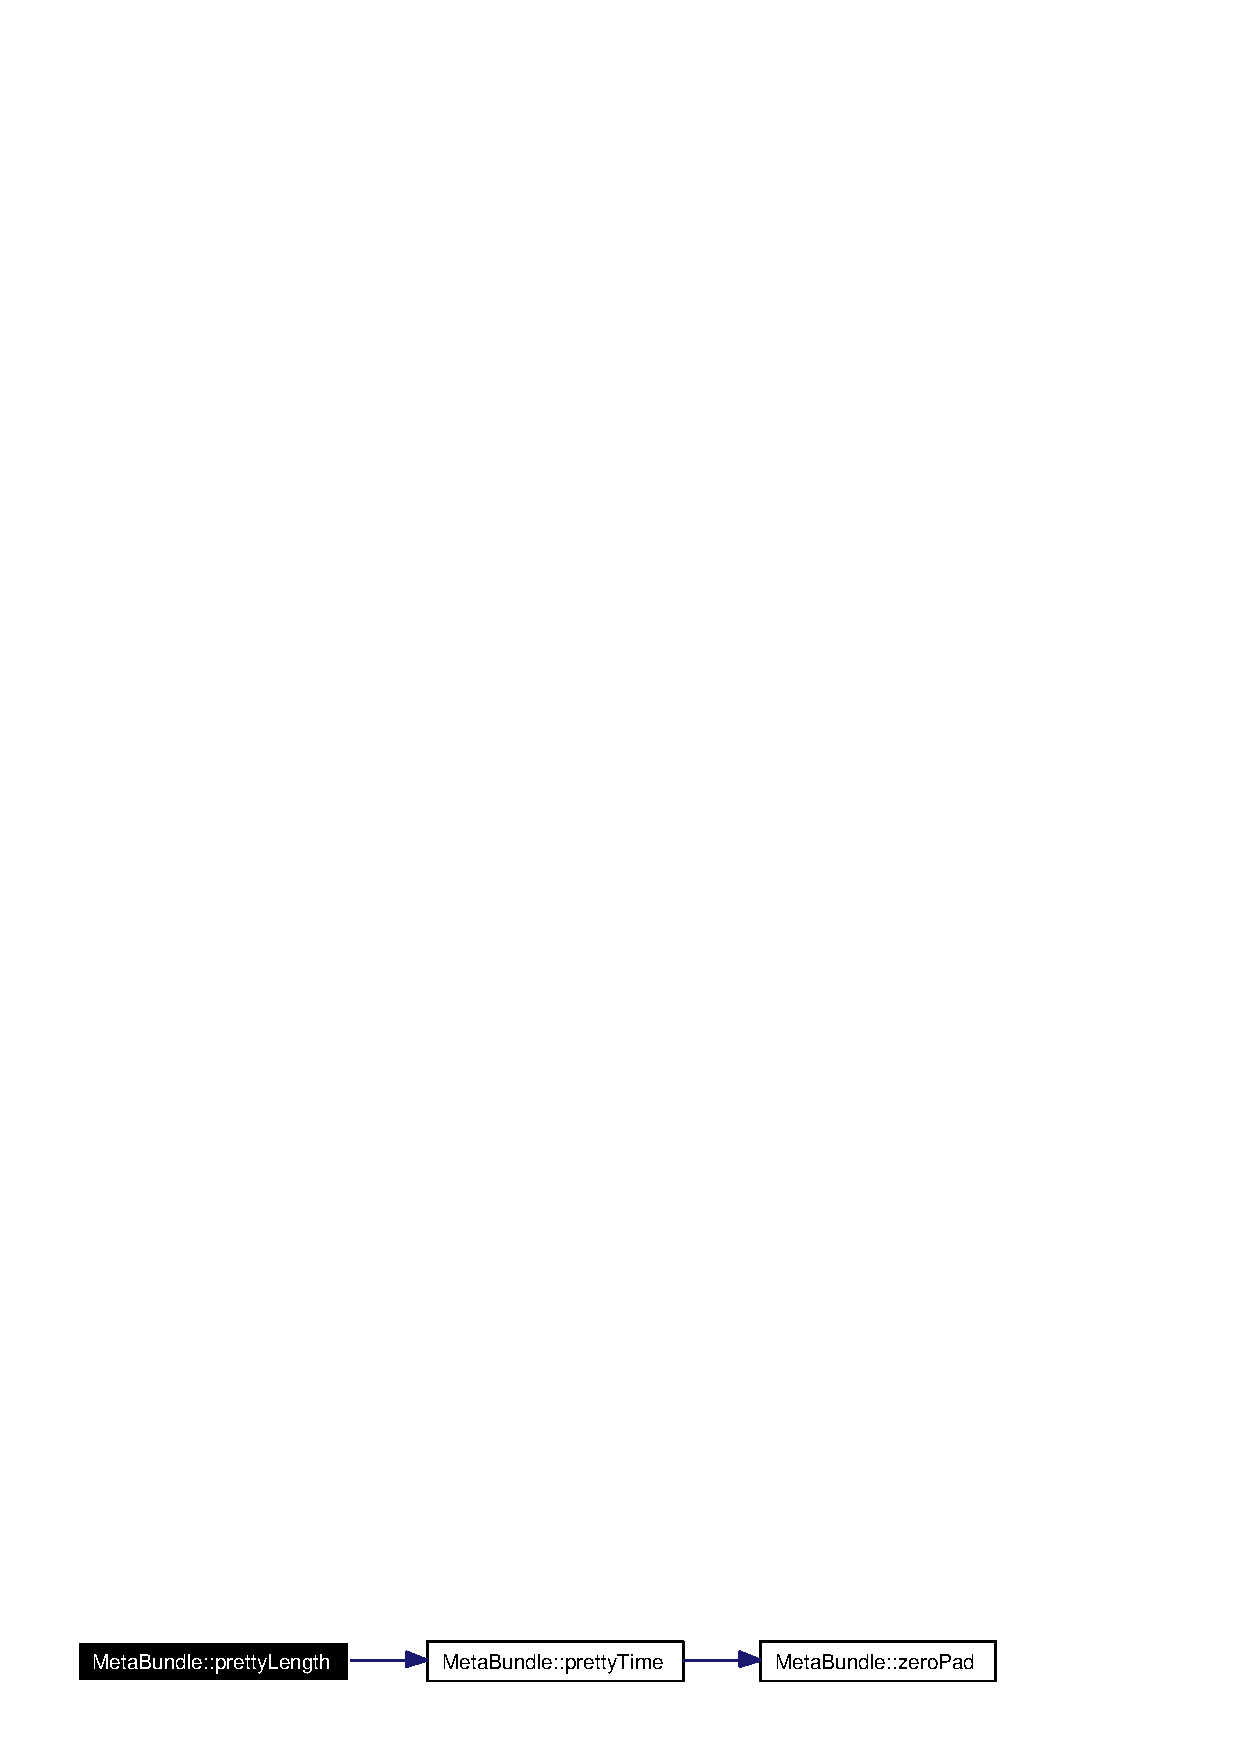
\includegraphics[width=239pt]{classMetaBundle_MetaBundlee1_cgraph}
\end{center}
\end{figure}
\index{MetaBundle@{Meta\-Bundle}!prettyLength@{prettyLength}}
\index{prettyLength@{prettyLength}!MetaBundle@{Meta\-Bundle}}
\subsubsection{\setlength{\rightskip}{0pt plus 5cm}QString Meta\-Bundle::pretty\-Length () const\hspace{0.3cm}{\tt  [inline]}}\label{classMetaBundle_MetaBundlea20}




Definition at line 70 of file metabundle.h.

References m\_\-length.



\footnotesize\begin{verbatim}70 { return prettyLength( m_length ); }
\end{verbatim}\normalsize 
\index{MetaBundle@{Meta\-Bundle}!prettySampleRate@{prettySampleRate}}
\index{prettySampleRate@{prettySampleRate}!MetaBundle@{Meta\-Bundle}}
\subsubsection{\setlength{\rightskip}{0pt plus 5cm}QString Meta\-Bundle::pretty\-Sample\-Rate () const\hspace{0.3cm}{\tt  [inline]}}\label{classMetaBundle_MetaBundlea21}




Definition at line 71 of file metabundle.h.

References m\_\-sample\-Rate, and pretty\-Generic().



\footnotesize\begin{verbatim}71 { return prettyGeneric( i18n( "SampleRate", "%1 Hz" ), m_sampleRate ); }
\end{verbatim}\normalsize 


Here is the call graph for this function:\begin{figure}[H]
\begin{center}
\leavevmode

\includegraphics[width=182pt]{classMetaBundle_MetaBundlea21_cgraph}
\end{center}
\end{figure}
\index{MetaBundle@{Meta\-Bundle}!prettyTime@{prettyTime}}
\index{prettyTime@{prettyTime}!MetaBundle@{Meta\-Bundle}}
\subsubsection{\setlength{\rightskip}{0pt plus 5cm}QString Meta\-Bundle::pretty\-Time (int, bool {\em show\-Hours} = true)\hspace{0.3cm}{\tt  [static]}}\label{classMetaBundle_MetaBundlee2}




Definition at line 224 of file metabundle.cpp.

References zero\-Pad().

Referenced by pretty\-Length().



\footnotesize\begin{verbatim}225 {
226     QString s = QChar( ':' );
227     s.append( zeroPad( seconds % 60 ) ); //seconds
228     seconds /= 60;
229 
230     if( showHours )
231     {
232         s.prepend( zeroPad( seconds % 60 ) ); //minutes
233         s.prepend( ':' );
234         seconds /= 60;
235     }
236 
237     //don't zeroPad the last one, as it can be greater than 2 digits
238     s.prepend( QString::number( seconds ) ); //hours or minutes depending on above if block
239 
240     return s;
241 }
\end{verbatim}\normalsize 


Here is the call graph for this function:\begin{figure}[H]
\begin{center}
\leavevmode

\includegraphics[width=155pt]{classMetaBundle_MetaBundlee2_cgraph}
\end{center}
\end{figure}
\index{MetaBundle@{Meta\-Bundle}!prettyTitle@{prettyTitle}}
\index{prettyTitle@{prettyTitle}!MetaBundle@{Meta\-Bundle}}
\subsubsection{\setlength{\rightskip}{0pt plus 5cm}QString Meta\-Bundle::pretty\-Title (QString)\hspace{0.3cm}{\tt  [static]}}\label{classMetaBundle_MetaBundlee4}




Definition at line 200 of file metabundle.cpp.



\footnotesize\begin{verbatim}201 {
202     QString &s = filename; //just so the code is more readable
203 
204     //remove file extension, s/_/ /g and decode %2f-like sequences
205     s = s.left( s.findRev( '.' ) ).replace( '_', ' ' );
206     s = KURL::decode_string(s);
207 
208     return s;
209 }
\end{verbatim}\normalsize 
\index{MetaBundle@{Meta\-Bundle}!prettyTitle@{prettyTitle}}
\index{prettyTitle@{prettyTitle}!MetaBundle@{Meta\-Bundle}}
\subsubsection{\setlength{\rightskip}{0pt plus 5cm}QString Meta\-Bundle::pretty\-Title () const}\label{classMetaBundle_MetaBundlea17}




Definition at line 187 of file metabundle.cpp.

References m\_\-artist, m\_\-title, and m\_\-url.

Referenced by init().



\footnotesize\begin{verbatim}188 {
189     //NOTE this gets regressed often, please be careful!
190     //NOTE whatever you do, handle the stream case, streams have no artist but have an excellent title
191 
192     QString s = m_artist;
193     if( !s.isEmpty() ) s += " - ";
194     s += m_title;
195     if( s.isEmpty() ) s = prettyTitle( m_url.fileName() );
196     return s;
197 }
\end{verbatim}\normalsize 
\index{MetaBundle@{Meta\-Bundle}!prettyURL@{prettyURL}}
\index{prettyURL@{prettyURL}!MetaBundle@{Meta\-Bundle}}
\subsubsection{\setlength{\rightskip}{0pt plus 5cm}QString Meta\-Bundle::pretty\-URL () const\hspace{0.3cm}{\tt  [inline]}}\label{classMetaBundle_MetaBundlea18}




Definition at line 68 of file metabundle.h.

References m\_\-url.



\footnotesize\begin{verbatim}68 { return m_url.prettyURL(); }
\end{verbatim}\normalsize 
\index{MetaBundle@{Meta\-Bundle}!readTags@{readTags}}
\index{readTags@{readTags}!MetaBundle@{Meta\-Bundle}}
\subsubsection{\setlength{\rightskip}{0pt plus 5cm}{\bf Meta\-Bundle} \& Meta\-Bundle::read\-Tags (bool {\em audio\-Properties} = true)}\label{classMetaBundle_MetaBundlea4}




Definition at line 159 of file metabundle.cpp.

References init(), m\_\-album, m\_\-artist, m\_\-comment, m\_\-genre, m\_\-title, m\_\-track, m\_\-url, and m\_\-year.

Referenced by Meta\-Bundle().



\footnotesize\begin{verbatim}160 {
161     //TODO detect mimetype and use specfic reader like Scott recommends
162 
163    TagLib::FileRef f( m_url.path().local8Bit(), audioProperties, TagLib::AudioProperties::Fast );
164 
165    if ( !f.isNull() )
166    {
167         if( f.tag() )
168         {
169             TagLib::Tag *tag = f.tag();
170 
171             m_title   = TStringToQString( tag->title() ).stripWhiteSpace();
172             m_artist  = TStringToQString( tag->artist() ).stripWhiteSpace();
173             m_album   = TStringToQString( tag->album() ).stripWhiteSpace();
174             m_comment = TStringToQString( tag->comment() ).stripWhiteSpace();
175             m_genre   = TStringToQString( tag->genre() ).stripWhiteSpace();
176             m_year    = tag->year() ? QString::number( tag->year() ) : QString::null;
177             m_track   = tag->track() ? QString::number( tag->track() ) : QString::null;
178         }
179         init( f.audioProperties() );
180     }
181     else init( KFileMetaInfo( m_url, QString::null, KFileMetaInfo::Everything ) );
182 
183     return *this;
184 }
\end{verbatim}\normalsize 


Here is the call graph for this function:\begin{figure}[H]
\begin{center}
\leavevmode

\includegraphics[width=139pt]{classMetaBundle_MetaBundlea4_cgraph}
\end{center}
\end{figure}
\index{MetaBundle@{Meta\-Bundle}!sampleRate@{sampleRate}}
\index{sampleRate@{sampleRate}!MetaBundle@{Meta\-Bundle}}
\subsubsection{\setlength{\rightskip}{0pt plus 5cm}int Meta\-Bundle::sample\-Rate () const\hspace{0.3cm}{\tt  [inline]}}\label{classMetaBundle_MetaBundlea7}




Definition at line 56 of file metabundle.h.

References m\_\-sample\-Rate.



\footnotesize\begin{verbatim}56 { return m_sampleRate; }
\end{verbatim}\normalsize 
\index{MetaBundle@{Meta\-Bundle}!title@{title}}
\index{title@{title}!MetaBundle@{Meta\-Bundle}}
\subsubsection{\setlength{\rightskip}{0pt plus 5cm}const QString\& Meta\-Bundle::title () const\hspace{0.3cm}{\tt  [inline]}}\label{classMetaBundle_MetaBundlea10}




Definition at line 59 of file metabundle.h.

References m\_\-title.

Referenced by Myplayer::handle\-Message().



\footnotesize\begin{verbatim}59 { return m_title; }
\end{verbatim}\normalsize 
\index{MetaBundle@{Meta\-Bundle}!track@{track}}
\index{track@{track}!MetaBundle@{Meta\-Bundle}}
\subsubsection{\setlength{\rightskip}{0pt plus 5cm}const QString\& Meta\-Bundle::track () const\hspace{0.3cm}{\tt  [inline]}}\label{classMetaBundle_MetaBundlea16}




Definition at line 65 of file metabundle.h.

References m\_\-track.



\footnotesize\begin{verbatim}65 { return m_track; }
\end{verbatim}\normalsize 
\index{MetaBundle@{Meta\-Bundle}!url@{url}}
\index{url@{url}!MetaBundle@{Meta\-Bundle}}
\subsubsection{\setlength{\rightskip}{0pt plus 5cm}const KURL\& Meta\-Bundle::url () const\hspace{0.3cm}{\tt  [inline]}}\label{classMetaBundle_MetaBundlea9}




Definition at line 58 of file metabundle.h.

References m\_\-url.

Referenced by Engine\-Controller::play().



\footnotesize\begin{verbatim}58 { return m_url; }
\end{verbatim}\normalsize 
\index{MetaBundle@{Meta\-Bundle}!year@{year}}
\index{year@{year}!MetaBundle@{Meta\-Bundle}}
\subsubsection{\setlength{\rightskip}{0pt plus 5cm}const QString\& Meta\-Bundle::year () const\hspace{0.3cm}{\tt  [inline]}}\label{classMetaBundle_MetaBundlea13}




Definition at line 62 of file metabundle.h.

References m\_\-year.



\footnotesize\begin{verbatim}62 { return m_year; }
\end{verbatim}\normalsize 
\index{MetaBundle@{Meta\-Bundle}!zeroPad@{zeroPad}}
\index{zeroPad@{zeroPad}!MetaBundle@{Meta\-Bundle}}
\subsubsection{\setlength{\rightskip}{0pt plus 5cm}QString Meta\-Bundle::zero\-Pad (uint {\em i})\hspace{0.3cm}{\tt  [inline, static]}}\label{classMetaBundle_MetaBundlee3}




Definition at line 76 of file metabundle.h.

Referenced by pretty\-Time().



\footnotesize\begin{verbatim}76 { return ( i < 10 ) ? QString( "0%1" ).arg( i ) : QString::number( i ); }
\end{verbatim}\normalsize 


\subsection{Member Data Documentation}
\index{MetaBundle@{Meta\-Bundle}!exists@{exists}}
\index{exists@{exists}!MetaBundle@{Meta\-Bundle}}
\subsubsection{\setlength{\rightskip}{0pt plus 5cm}bool {\bf Meta\-Bundle::exists}\hspace{0.3cm}{\tt  [private]}}\label{classMetaBundle_MetaBundler11}




Definition at line 101 of file metabundle.h.

Referenced by exist(), and init().\index{MetaBundle@{Meta\-Bundle}!Irrelevant@{Irrelevant}}
\index{Irrelevant@{Irrelevant}!MetaBundle@{Meta\-Bundle}}
\subsubsection{\setlength{\rightskip}{0pt plus 5cm}const int {\bf Meta\-Bundle::Irrelevant} = -1\hspace{0.3cm}{\tt  [static]}}\label{classMetaBundle_MetaBundles1}




Definition at line 29 of file metabundle.h.

Referenced by pretty\-Length().\index{MetaBundle@{Meta\-Bundle}!m_album@{m\_\-album}}
\index{m_album@{m\_\-album}!MetaBundle@{Meta\-Bundle}}
\subsubsection{\setlength{\rightskip}{0pt plus 5cm}QString {\bf Meta\-Bundle::m\_\-album}\hspace{0.3cm}{\tt  [private]}}\label{classMetaBundle_MetaBundler3}




Definition at line 83 of file metabundle.h.

Referenced by album(), init(), and read\-Tags().\index{MetaBundle@{Meta\-Bundle}!m_artist@{m\_\-artist}}
\index{m_artist@{m\_\-artist}!MetaBundle@{Meta\-Bundle}}
\subsubsection{\setlength{\rightskip}{0pt plus 5cm}QString {\bf Meta\-Bundle::m\_\-artist}\hspace{0.3cm}{\tt  [private]}}\label{classMetaBundle_MetaBundler2}




Definition at line 82 of file metabundle.h.

Referenced by artist(), init(), pretty\-Title(), and read\-Tags().\index{MetaBundle@{Meta\-Bundle}!m_bitrate@{m\_\-bitrate}}
\index{m_bitrate@{m\_\-bitrate}!MetaBundle@{Meta\-Bundle}}
\subsubsection{\setlength{\rightskip}{0pt plus 5cm}int {\bf Meta\-Bundle::m\_\-bitrate}\hspace{0.3cm}{\tt  [private]}}\label{classMetaBundle_MetaBundler8}




Definition at line 93 of file metabundle.h.

Referenced by bitrate(), init(), and pretty\-Bitrate().\index{MetaBundle@{Meta\-Bundle}!m_comment@{m\_\-comment}}
\index{m_comment@{m\_\-comment}!MetaBundle@{Meta\-Bundle}}
\subsubsection{\setlength{\rightskip}{0pt plus 5cm}QString {\bf Meta\-Bundle::m\_\-comment}\hspace{0.3cm}{\tt  [private]}}\label{classMetaBundle_MetaBundler5}




Definition at line 85 of file metabundle.h.

Referenced by comment(), init(), and read\-Tags().\index{MetaBundle@{Meta\-Bundle}!m_genre@{m\_\-genre}}
\index{m_genre@{m\_\-genre}!MetaBundle@{Meta\-Bundle}}
\subsubsection{\setlength{\rightskip}{0pt plus 5cm}QString {\bf Meta\-Bundle::m\_\-genre}\hspace{0.3cm}{\tt  [private]}}\label{classMetaBundle_MetaBundler6}




Definition at line 86 of file metabundle.h.

Referenced by genre(), init(), and read\-Tags().\index{MetaBundle@{Meta\-Bundle}!m_length@{m\_\-length}}
\index{m_length@{m\_\-length}!MetaBundle@{Meta\-Bundle}}
\subsubsection{\setlength{\rightskip}{0pt plus 5cm}int {\bf Meta\-Bundle::m\_\-length}\hspace{0.3cm}{\tt  [private]}}\label{classMetaBundle_MetaBundler9}




Definition at line 94 of file metabundle.h.

Referenced by init(), length(), and pretty\-Length().\index{MetaBundle@{Meta\-Bundle}!m_sampleRate@{m\_\-sampleRate}}
\index{m_sampleRate@{m\_\-sampleRate}!MetaBundle@{Meta\-Bundle}}
\subsubsection{\setlength{\rightskip}{0pt plus 5cm}int {\bf Meta\-Bundle::m\_\-sample\-Rate}\hspace{0.3cm}{\tt  [private]}}\label{classMetaBundle_MetaBundler10}




Definition at line 95 of file metabundle.h.

Referenced by init(), pretty\-Sample\-Rate(), and sample\-Rate().\index{MetaBundle@{Meta\-Bundle}!m_title@{m\_\-title}}
\index{m_title@{m\_\-title}!MetaBundle@{Meta\-Bundle}}
\subsubsection{\setlength{\rightskip}{0pt plus 5cm}QString {\bf Meta\-Bundle::m\_\-title}\hspace{0.3cm}{\tt  [private]}}\label{classMetaBundle_MetaBundler1}




Definition at line 81 of file metabundle.h.

Referenced by init(), pretty\-Title(), read\-Tags(), and title().\index{MetaBundle@{Meta\-Bundle}!m_track@{m\_\-track}}
\index{m_track@{m\_\-track}!MetaBundle@{Meta\-Bundle}}
\subsubsection{\setlength{\rightskip}{0pt plus 5cm}QString {\bf Meta\-Bundle::m\_\-track}\hspace{0.3cm}{\tt  [private]}}\label{classMetaBundle_MetaBundler7}




Definition at line 87 of file metabundle.h.

Referenced by init(), read\-Tags(), and track().\index{MetaBundle@{Meta\-Bundle}!m_url@{m\_\-url}}
\index{m_url@{m\_\-url}!MetaBundle@{Meta\-Bundle}}
\subsubsection{\setlength{\rightskip}{0pt plus 5cm}KURL {\bf Meta\-Bundle::m\_\-url}\hspace{0.3cm}{\tt  [private]}}\label{classMetaBundle_MetaBundler0}




Definition at line 80 of file metabundle.h.

Referenced by init(), Meta\-Bundle(), pretty\-Title(), pretty\-URL(), read\-Tags(), and url().\index{MetaBundle@{Meta\-Bundle}!m_year@{m\_\-year}}
\index{m_year@{m\_\-year}!MetaBundle@{Meta\-Bundle}}
\subsubsection{\setlength{\rightskip}{0pt plus 5cm}QString {\bf Meta\-Bundle::m\_\-year}\hspace{0.3cm}{\tt  [private]}}\label{classMetaBundle_MetaBundler4}




Definition at line 84 of file metabundle.h.

Referenced by init(), read\-Tags(), and year().\index{MetaBundle@{Meta\-Bundle}!Unavailable@{Unavailable}}
\index{Unavailable@{Unavailable}!MetaBundle@{Meta\-Bundle}}
\subsubsection{\setlength{\rightskip}{0pt plus 5cm}const int {\bf Meta\-Bundle::Unavailable} = 0\hspace{0.3cm}{\tt  [static]}}\label{classMetaBundle_MetaBundles2}




Definition at line 30 of file metabundle.h.

Referenced by pretty\-Length().\index{MetaBundle@{Meta\-Bundle}!Undetermined@{Undetermined}}
\index{Undetermined@{Undetermined}!MetaBundle@{Meta\-Bundle}}
\subsubsection{\setlength{\rightskip}{0pt plus 5cm}const int {\bf Meta\-Bundle::Undetermined} = -2\hspace{0.3cm}{\tt  [static]}}\label{classMetaBundle_MetaBundles0}




Definition at line 28 of file metabundle.h.

Referenced by init(), and pretty\-Generic().

The documentation for this class was generated from the following files:\begin{CompactItemize}
\item 
{\bf metabundle.h}\item 
{\bf metabundle.cpp}\end{CompactItemize}
